\documentclass[aspectratio=1610]{beamer}
\usepackage[utf8]{inputenc}
\usepackage[T1]{fontenc}
\usepackage{graphicx}
\usetheme{ulund}
\title{Decoding Sustainability\\Communication via NLP}
\author{nils.holmberg@iko.lu.se}
\begin{document}
\setbeamerfont{itemize/enumerate body}{size=\large}
\setbeamerfont{itemize/enumerate subbody}{size=\large}
\let\olditem\item
\renewcommand{\item}{\olditem\vspace{8pt}} % adjust to taste
\setlength{\itemsep}{8pt}  % spacing between items
\setlength{\parskip}{8pt}  % spacing between paragraphs (optional)

\begin{frame}[plain]
  \titlepage
\end{frame}

\begin{frame}
  \frametitle{Introduction}
  \begin{columns}[t]
    \begin{column}[t]{0.5\textwidth}
      \begin{itemize}
        \item Sustainability websites = transparency + persuasion
        \item Signal legitimacy and engage stakeholders
        \item Shell = technical; WWF = emotional
        \item Manual coding lacks scale/nuance
        \item \textbf{Aim:} Use NLP to compare Shell vs WWF
      \end{itemize}
    \end{column}
    \begin{column}[t]{0.5\textwidth}
      \vspace*{0pt}
      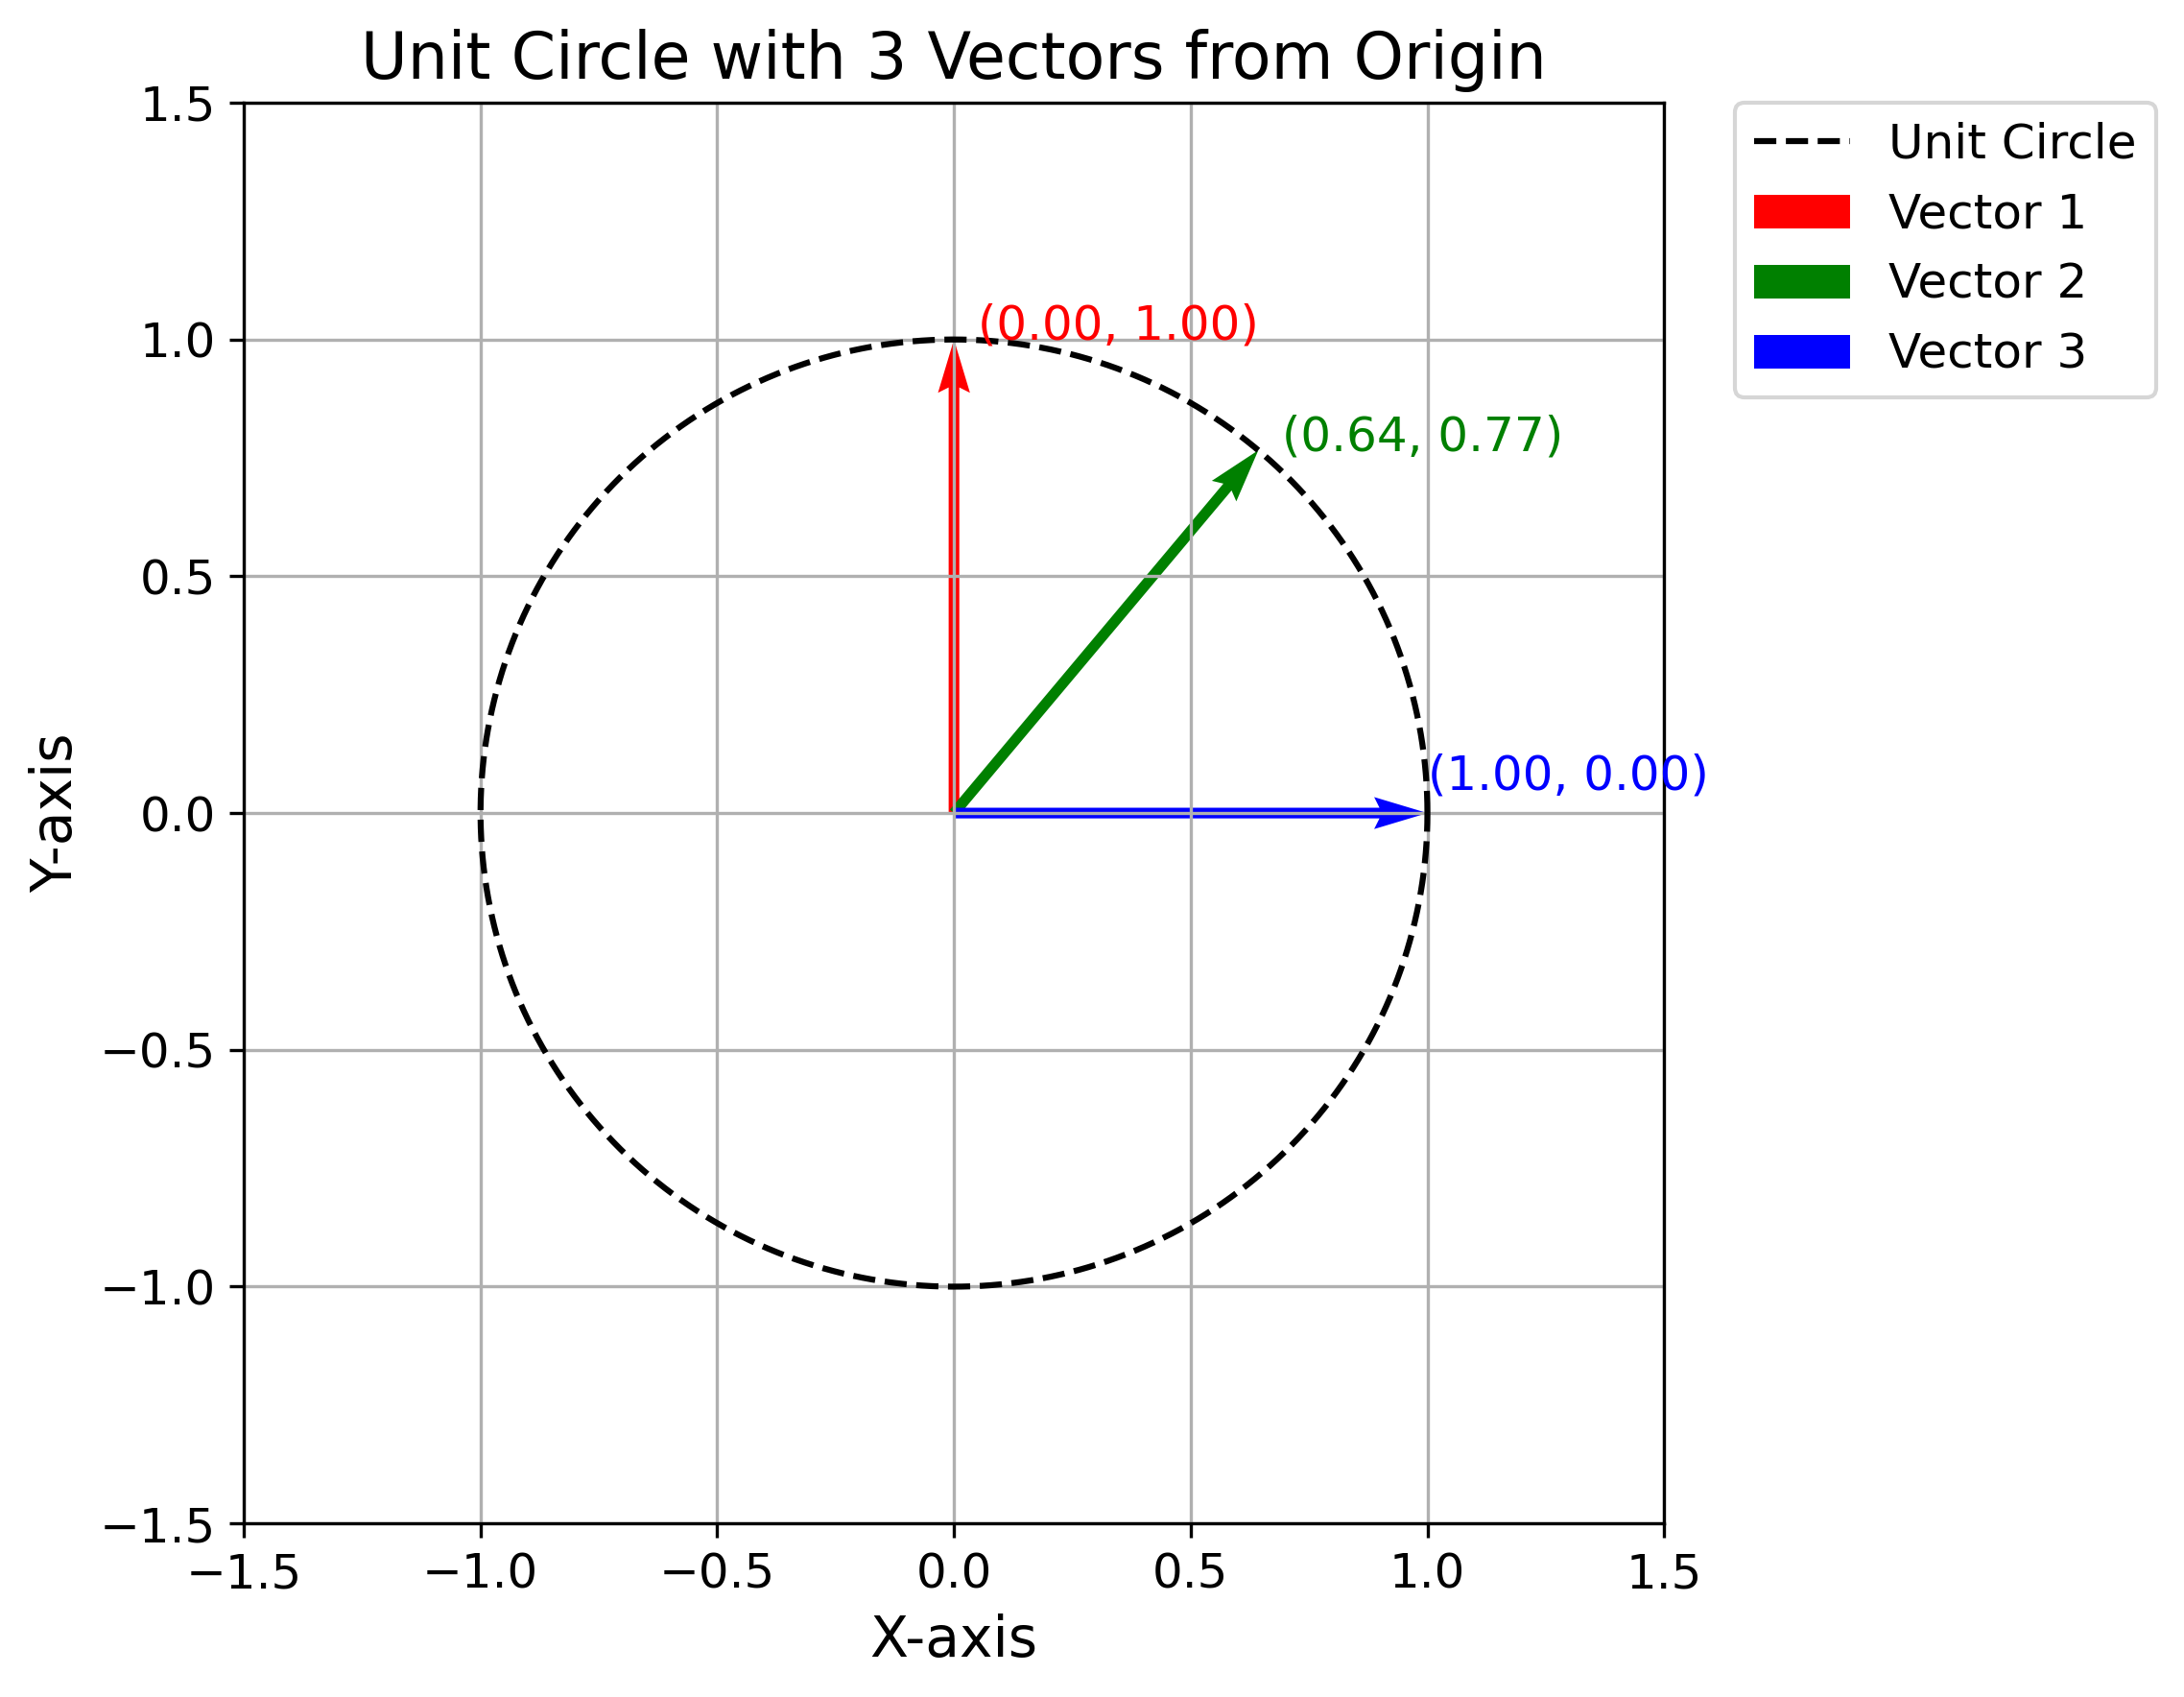
\includegraphics[width=\linewidth]{../../fig/unit_circle_vectors.png}
      (Insert diagram: corp vs NGO)
    \end{column}
  \end{columns}
\end{frame}

\begin{frame}
  \frametitle{Stakeholder Theory Expectations}
  \begin{columns}[t]
    \begin{column}[t]{0.6\textwidth}
      \begin{itemize}
        \item Message shaped by stakeholders
        \item Shell: investors/regulators = "investment", etc.
        \item WWF: donors/public = "donor", "nature"
        \item Shell: data-driven; WWF: community focus
        \item Predictable via lexical/semantic analysis
      \end{itemize}
    \end{column}
    \begin{column}[t]{0.4\textwidth}
      \vspace*{0pt}
      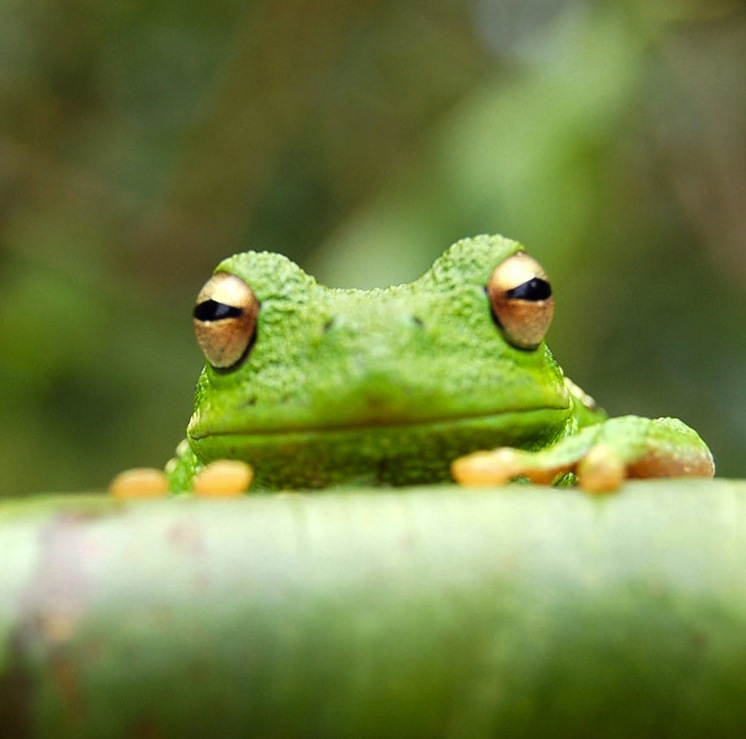
\includegraphics[width=\linewidth]{frog.jpg}
      (Insert graphic: stakeholder mapping)
    \end{column}
  \end{columns}
\end{frame}

\begin{frame}
  \frametitle{Framing Theory Expectations}
  \begin{columns}
    \begin{column}{0.6\textwidth}
      \begin{itemize}
        \item Framing guides perception
        \item Shell: optimistic "innovation" frame
        \item WWF: moral/problem frame ("action", "duty")
        \item Shell: business advantage; WWF: urgency
        \item Detectable via framing terms
      \end{itemize}
    \end{column}
    \begin{column}{0.4\textwidth}
      (Insert diagram: framing strategies)
    \end{column}
  \end{columns}
\end{frame}

\begin{frame}
  \frametitle{Data \& Methodology}
  \begin{columns}
    \begin{column}{0.6\textwidth}
      \begin{itemize}
        \item 7 webpages each from Shell and WWF
        \item Cleaned HTML, kept main content
        \item SpaCy tokenization, lemmatization
        \item Lexical: count theory-based keywords
        \item Semantic: BERT embeddings + similarity
      \end{itemize}
    \end{column}
    \begin{column}{0.4\textwidth}
      (Insert NLP pipeline sketch)
    \end{column}
  \end{columns}
\end{frame}

\begin{frame}
  \frametitle{Lexical Analysis Results}
  \begin{columns}
    \begin{column}{0.6\textwidth}
      \begin{itemize}
        \item Shell: "energy", "emission", "investment"
        \item WWF: "conservation", "donor", "nature"
        \item Terms rarely overlap between orgs
        \item Shell = tech \& opportunity; WWF = duty \& action
        \item Clear lexical patterns match theory
      \end{itemize}
    \end{column}
    \begin{column}{0.4\textwidth}
      (Insert frequency bar chart)
    \end{column}
  \end{columns}
\end{frame}

\begin{frame}
  \frametitle{Semantic Similarity (BERT)}
  \begin{columns}
    \begin{column}{0.6\textwidth}
      \begin{itemize}
        \item Shell aligns with "investment", etc.
        \item WWF aligns with "donor", "action"
        \item Shell avg. stakeholder similarity = 0.26
        \item WWF avg. framing similarity = 0.25
        \item Semantic match confirms lexical trends
      \end{itemize}
    \end{column}
    \begin{column}{0.4\textwidth}
      (Insert similarity heatmap)
    \end{column}
  \end{columns}
\end{frame}

\begin{frame}
  \frametitle{Theoretical Implications}
  \begin{columns}
    \begin{column}{0.6\textwidth}
      \begin{itemize}
        \item Shell confirms stakeholder focus
        \item WWF shows moral advocacy focus
        \item Shell = opportunity frame; WWF = moral frame
        \item NLP helps refine both theories
        \item Empirical grounding boosts explanatory power
      \end{itemize}
    \end{column}
    \begin{column}{0.4\textwidth}
      (Insert concept map: theory + findings)
    \end{column}
  \end{columns}
\end{frame}

\begin{frame}
  \frametitle{Communication Implications}
  \begin{columns}
    \begin{column}{0.6\textwidth}
      \begin{itemize}
        \item Shell = competence; WWF = emotional appeal
        \item Tailored messaging for each audience
        \item NLP = replicable insight, not anecdotal
        \item Firms = clarify tech; NGOs = build urgency
        \item Messaging must match mission + audience
      \end{itemize}
    \end{column}
    \begin{column}{0.4\textwidth}
      (Insert icons: tech vs moral appeals)
    \end{column}
  \end{columns}
\end{frame}

\begin{frame}
  \frametitle{Scalable Analysis}
  \begin{columns}
    \begin{column}{0.6\textwidth}
      \begin{itemize}
        \item Method scales to 100s of sites
        \item Cloud + BERT = efficient workflows
        \item Topic models could reveal trends
        \item Text + image data can be fused
        \item Big data boosts theory + practice
      \end{itemize}
    \end{column}
    \begin{column}{0.4\textwidth}
      (Insert cloud or NLP infrastructure diagram)
    \end{column}
  \end{columns}
\end{frame}

\begin{frame}
  \frametitle{Conclusion \& Future Directions}
  \begin{columns}
    \begin{column}{0.6\textwidth}
      \begin{itemize}
        \item NLP reveals Shell vs WWF messaging logics
        \item Confirms stakeholder + framing theory
        \item Lexical + semantic = stronger analysis
        \item Actionable insights for communication design
        \item Future: multimodal + large-scale studies
      \end{itemize}
    \end{column}
    \begin{column}{0.4\textwidth}
      (Insert multimodal analysis diagram)
    \end{column}
  \end{columns}
\end{frame}

\end{document}
